As explained in the introduction,
a trade policy that led to a dispute (preferably called as \textit{Government Measure} in WTO DSB) is pretty much complicated as explicitly expressed by the Panel in Figure \ref{fig:complex-measure}.
To address this complexity,
members who raise the claim (preferably called \textit{complainant} in WTO DSB) usually cite multiple articles of the WTO agreements at the same time. For example, in the
\textit{US - Offset} case,
a group of complainants\footnote{Australia,
   Brazil,
   Chile,
   European Communities,
   India,
   Indonesia,
   Japan,
   Korea and Thailand}
cited articles as shown in Table \ref{xltabular:cited-article-for-us-offset} from the WTO agreements to claim its inconsistencies of \textit{Continued Dumping and Subsidy Act of 2000} (CDSOA) to those cited articles\footnote{It is worth noting that the WTO agreements comprises many different agreements covering each specific topic in trade such as \textit{Agreement on Anti-dumping, Agreement on Subsidies and Countervailing Measures, Agreement on Agriculture} and so on.}:
\\
\begin{table}[h]
   \setlength\tabcolsep{15pt}
   \begin{tabular}{ c | c }
       \hline
       \textbf{\normalsize Name of WTO Agreement}          & \textbf{\normalsize Cited Articles} \\
       \hline \hline
       Agreement on Anti-dumping                           & 1, 5.4, 8, 18.1, 18.4               \\ \hline
       General Agreement on Tariffs and Trade 1994         & VI:3, X:3, XXIII:1, VI:2            \\ \hline
       Agreement on Subsidies and Countervailing Measures  & 4.10, 7.9, 10, 11.4, 18, 32.1, 32.5 \\ \hline
       Agreement Establishing the World Trade Organization & XVI:4                               \\ \hline
   \end{tabular}
   \caption{Cited articles in \textit{US - Offset (Byrd Amendment)} by complainants}
   \label{xltabular:cited-article-for-us-offset}
\end{table}
 
\noindent Upon this understanding,
I collected two different types of data for 143 different dispute cases requested to WTO DSB. (List of cases is
available at \hyperref[sub:cited-articles-table]{Appendix A.2}).
One is textual description of the dispute \hyperref[sub:factual-aspect-example]{(\textit{Check} the CDSOA example at Appendix A.1)} and the other one is
set of articles of the WTO agreements that are
cited for each dispute \hyperref[sub:cited-articles-table]{(Appendix A.3)}.
I will explain the data source, structure and collection method for two different types of data at the following subsections.\\
 
\begin{figure}[h]
    \centering
    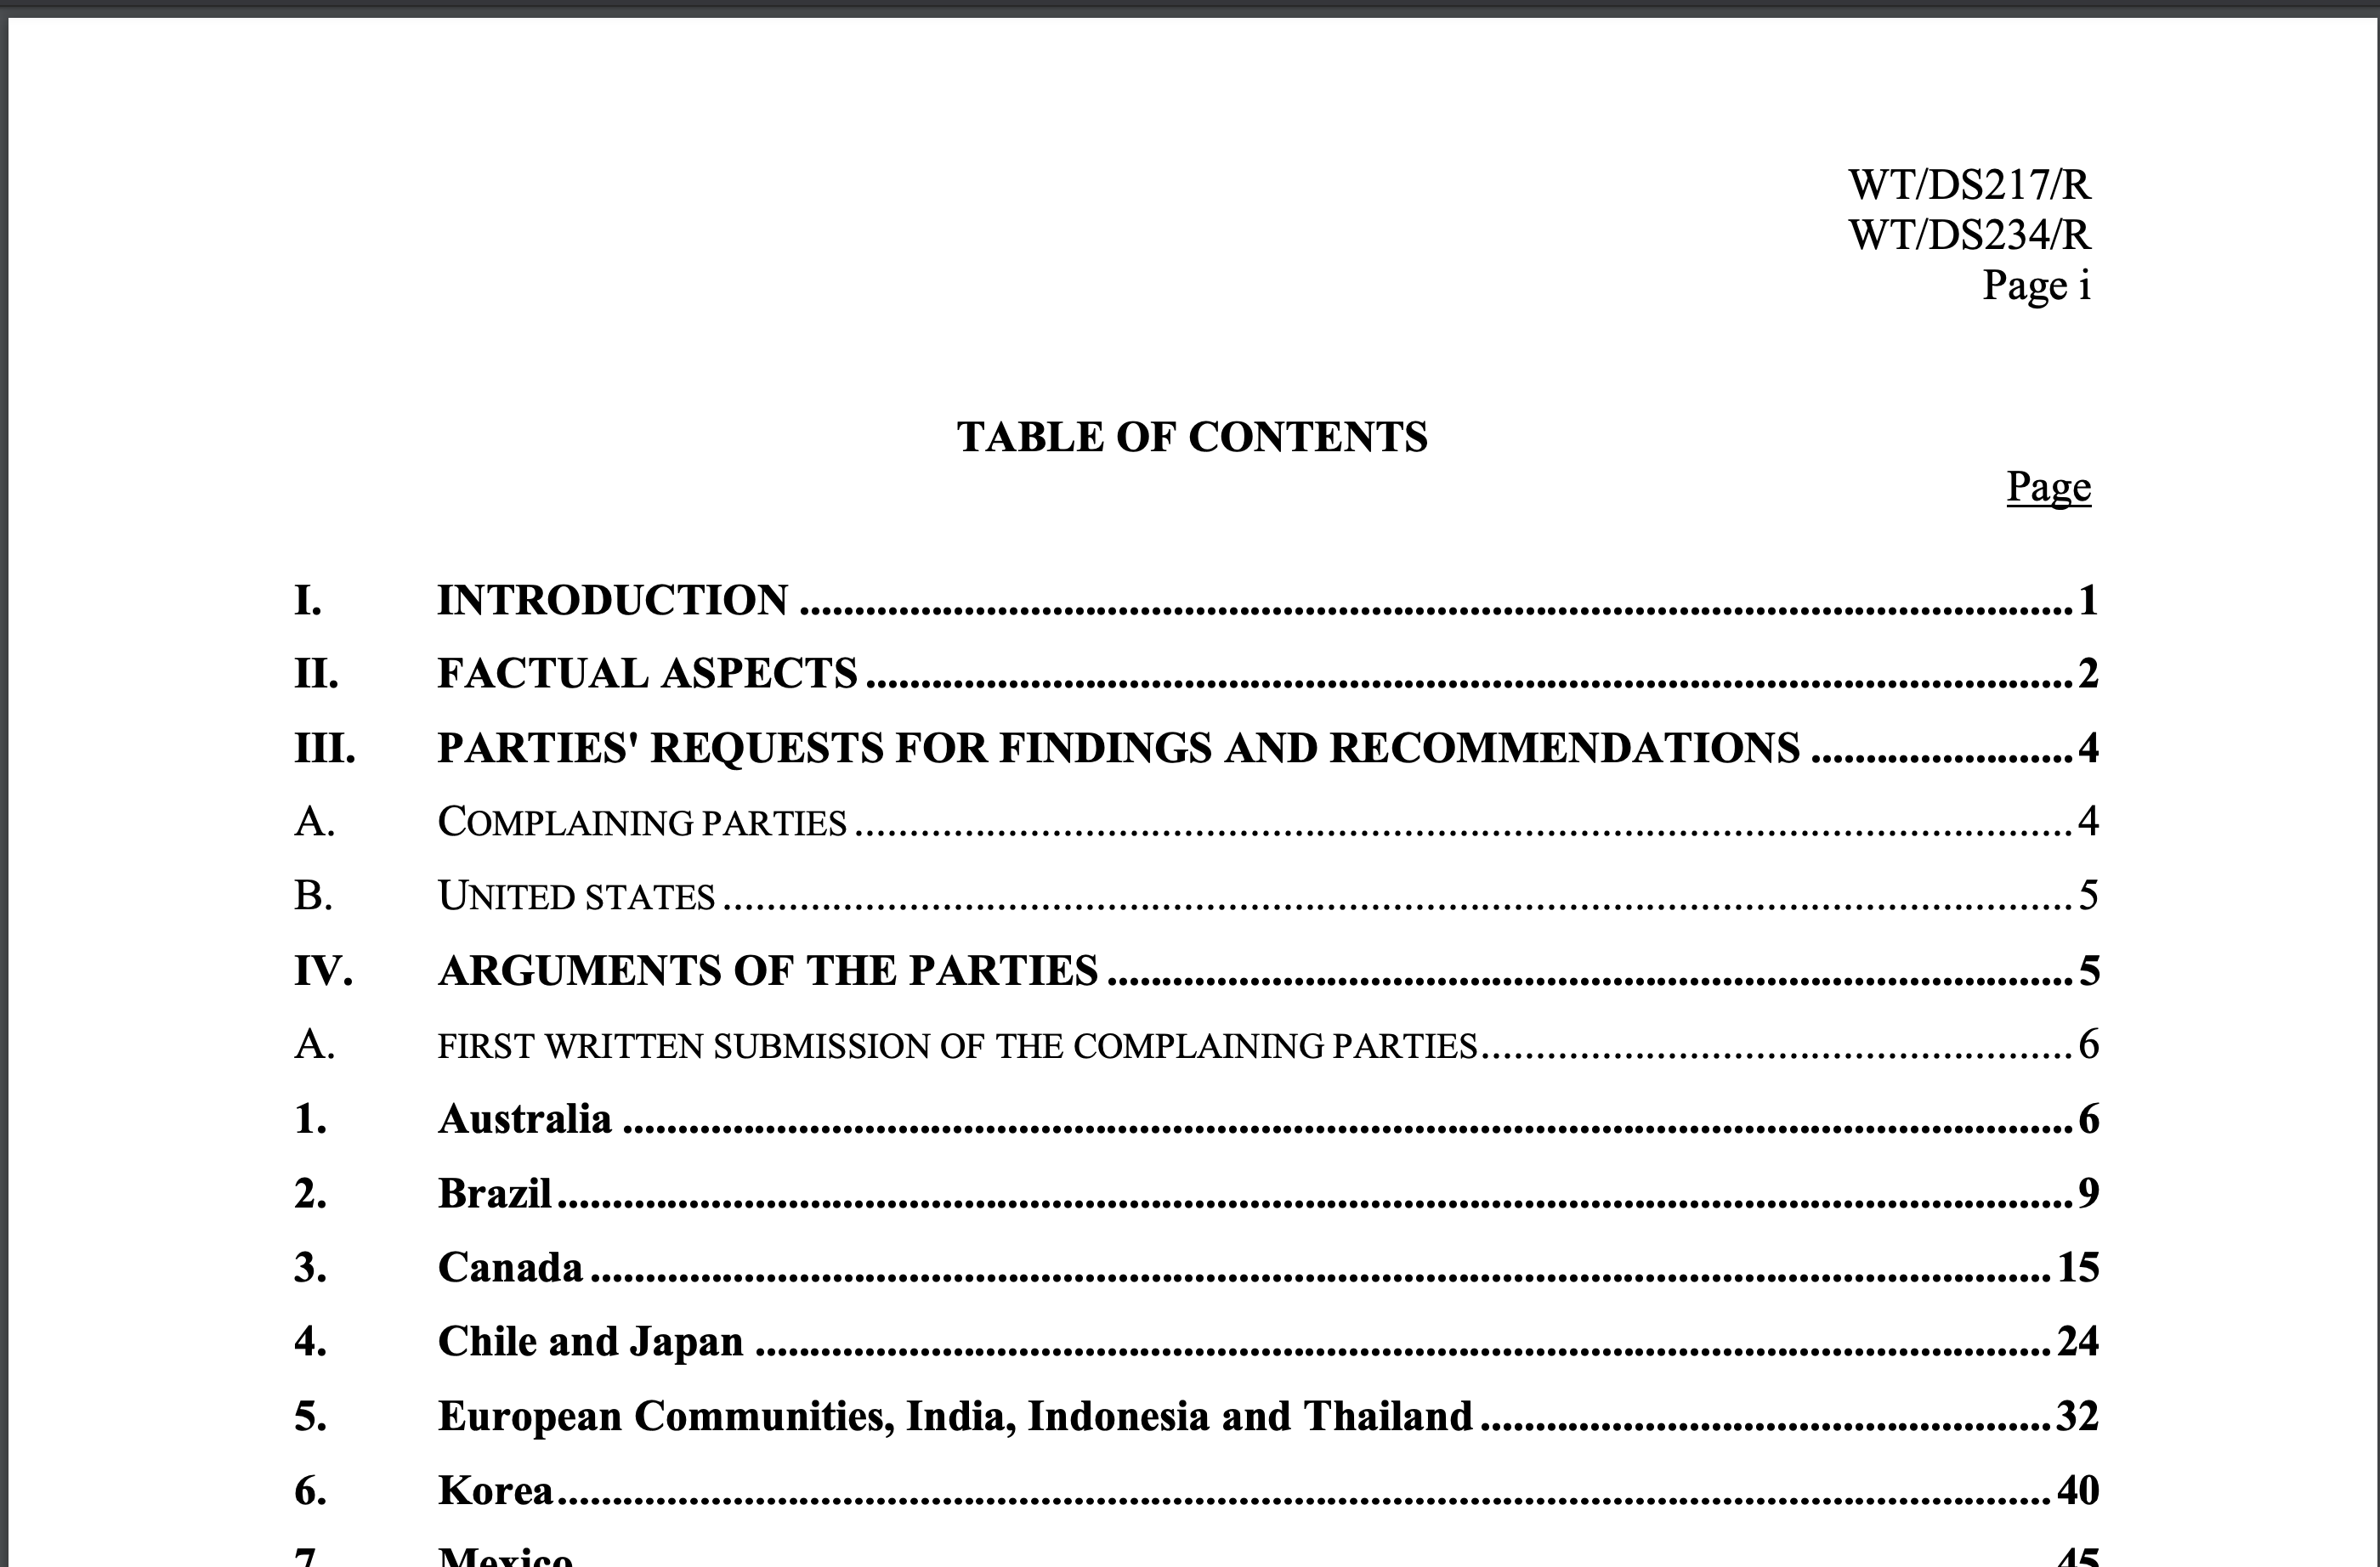
\includegraphics[scale=0.28]{Data/pngs/panel_report_toc.png}
    \caption{
        {\bf Table of Contents of Panel Report: }Panel provides 
        factual aspect in the panel report with its page location.
        }
    \label{fig:panel-report-toc}
\end{figure}
% \begin{center}
%     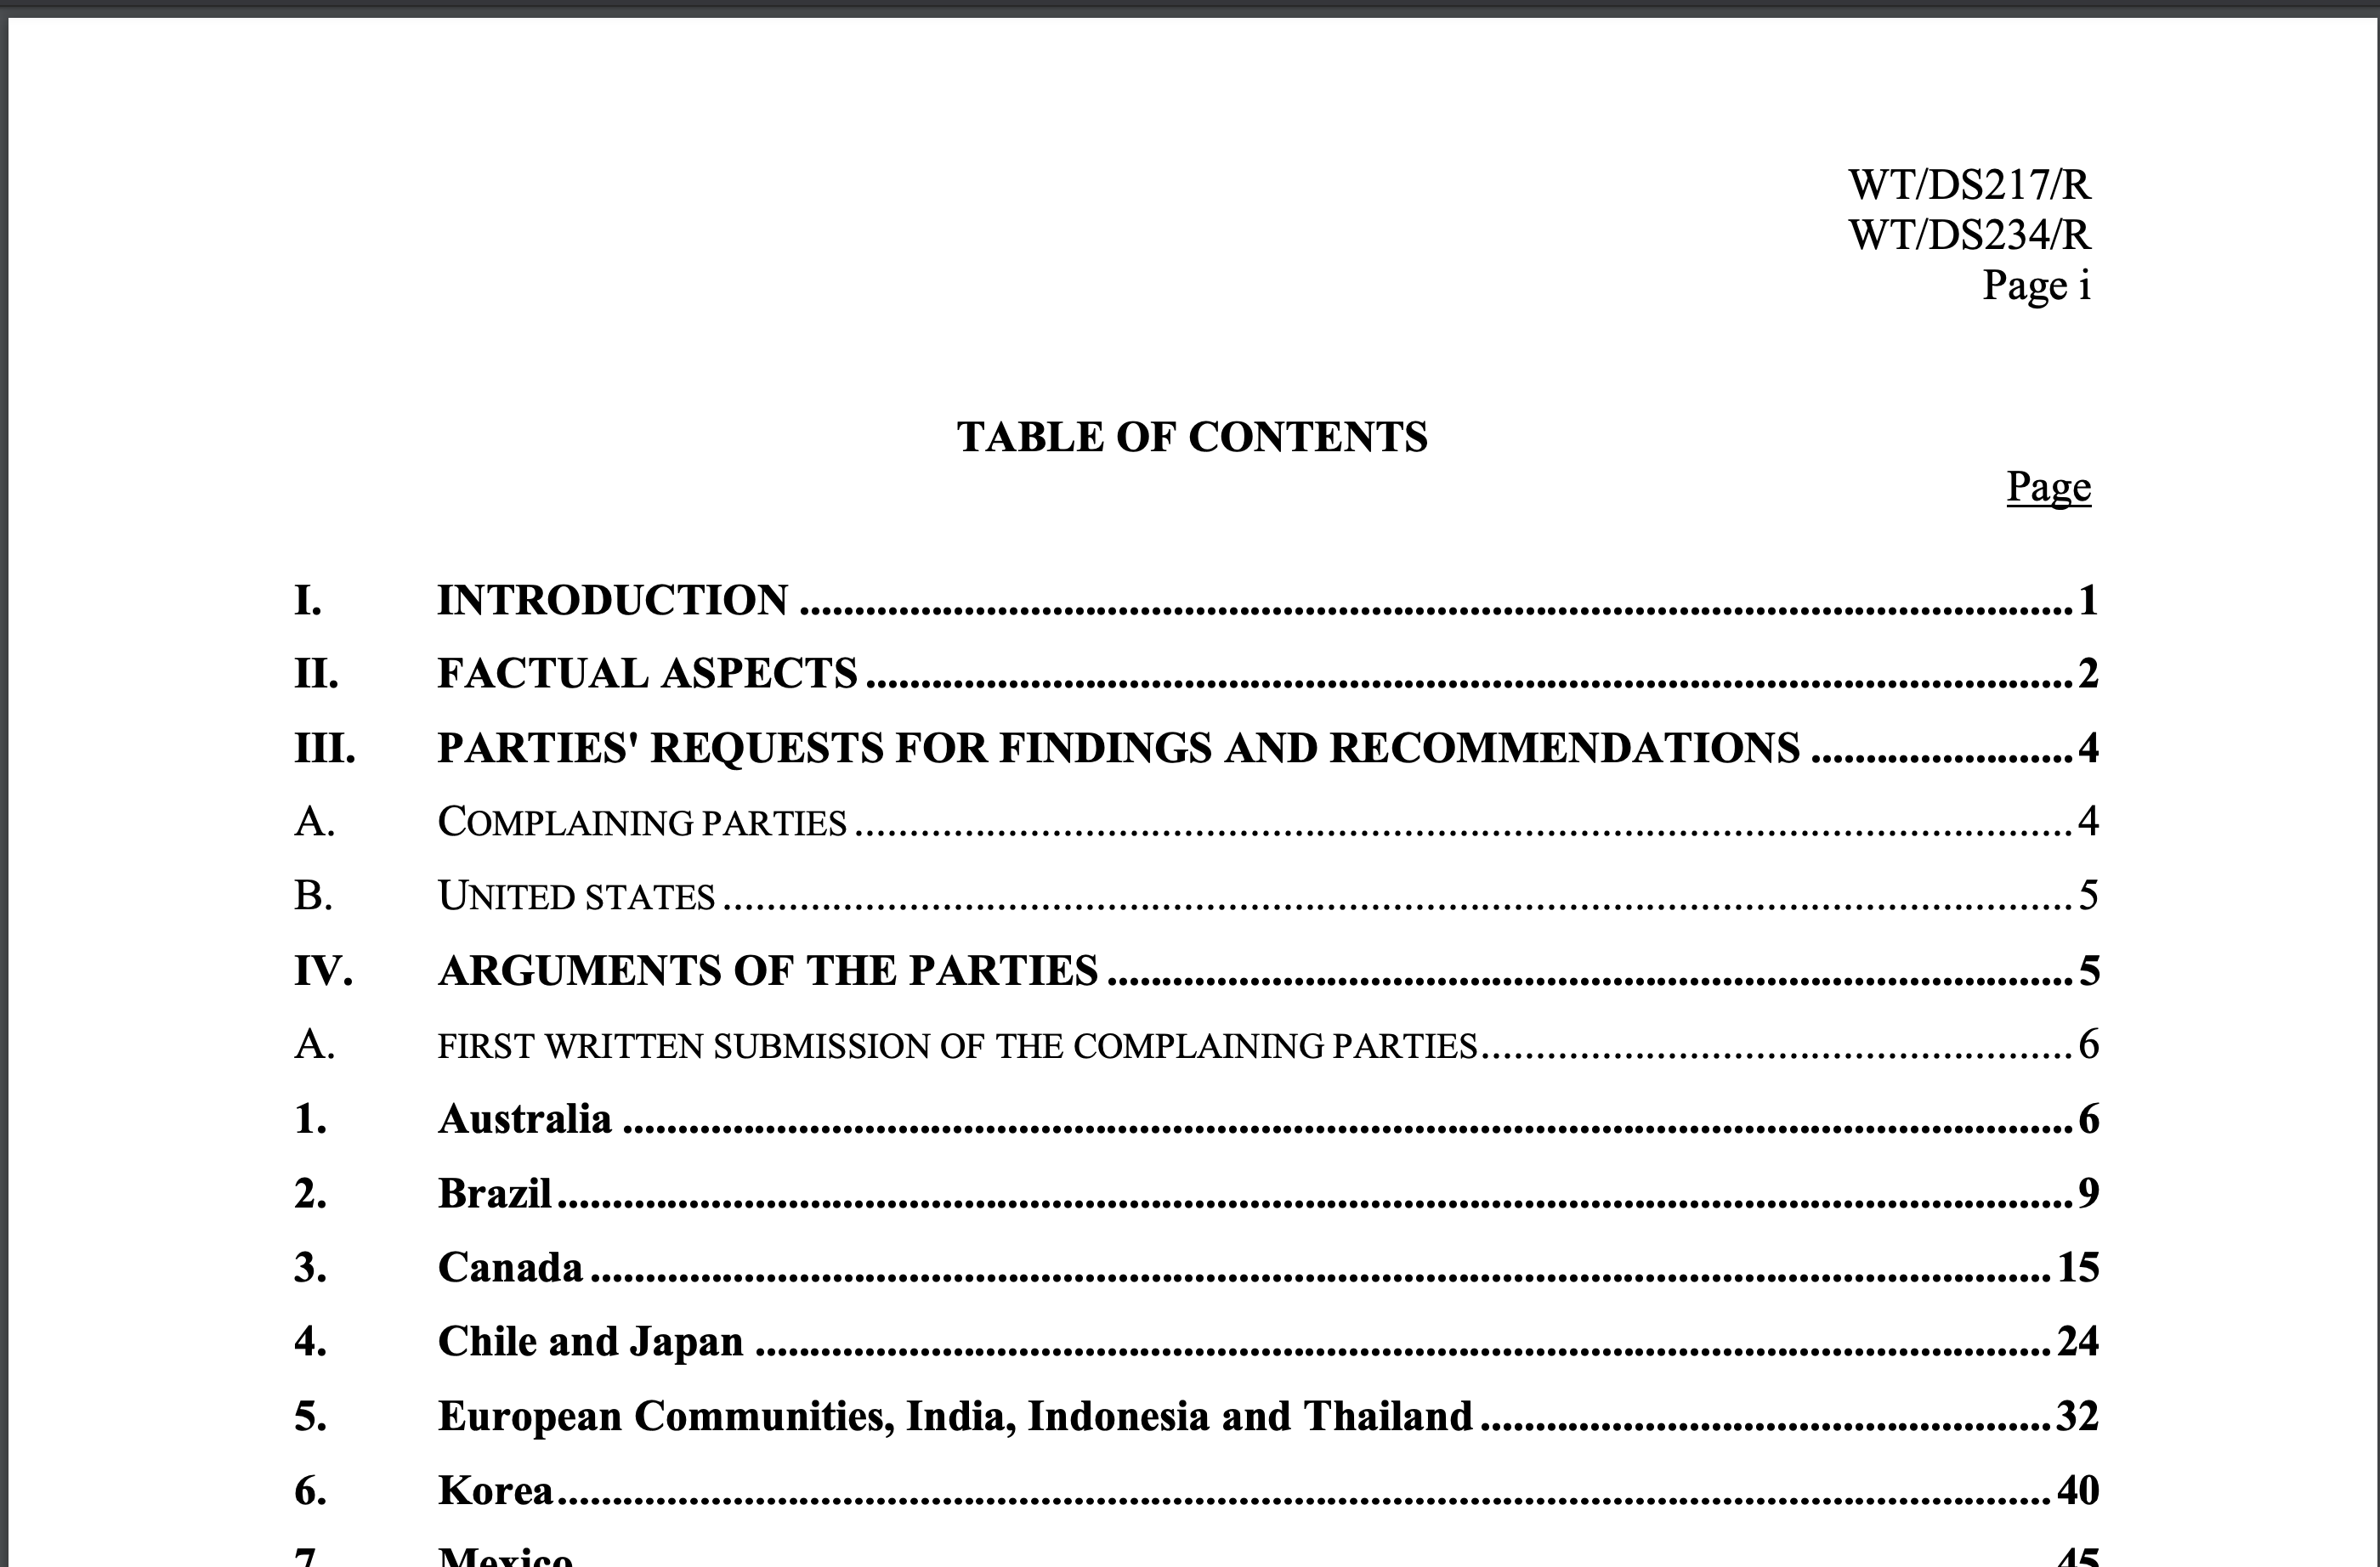
\includegraphics[scale=0.3]{Data/pngs/panel_report_toc.png}
% \end{center}

 
 

